33. $\cfrac{(-1+x^2)(1-x)^2(x+1)^3}{x^8-x^6+x^4}\leqslant0\Leftrightarrow\cfrac{(x-1)^3(x+1)^4}{x^4(x^4-x^2+1)}\leqslant0.$ Применив метод интервалов, найдём ответ: $x\in(-\infty;0)\cup(0;1].$
\begin{figure}[ht!]
\center{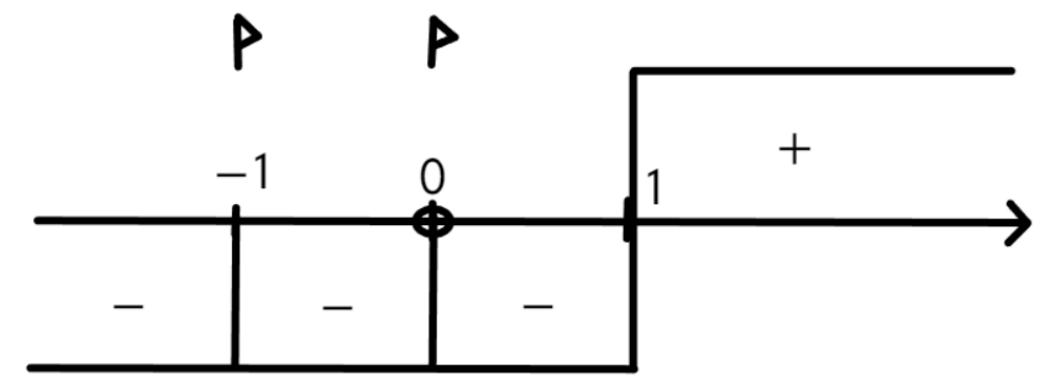
\includegraphics[scale=0.35]{ner9-33.png}}
\end{figure}\\
